\documentclass{article}

% if you need to pass options to natbib, use, e.g.:
% \PassOptionsToPackage{numbers, compress}{natbib}
% before loading nips_2016
%
% to avoid loading the natbib package, add option nonatbib:
% \usepackage[nonatbib]{nips_2016}

\usepackage[final]{nips_2016}

% to compile a camera-ready version, add the [final] option, e.g.:
% \usepackage[final]{nips_2016}

\usepackage[utf8]{inputenc} % allow utf-8 input
\usepackage[T1]{fontenc}    % use 8-bit T1 fonts
\usepackage{hyperref}       % hyperlinks
\usepackage{url}            % simple URL typesetting
\usepackage{booktabs}       % professional-quality tables
\usepackage{amsfonts}       % blackboard math symbols
%\usepackage{nicefrac}       % compact symbols for 1/2, etc.
\usepackage{microtype}      % microtypography

\usepackage{amssymb, amsmath}
\usepackage{epsfig}
\usepackage{array}
\usepackage{ifthen}
\usepackage{color}
\usepackage{fancyhdr}
\usepackage{graphicx}
\usepackage{mathtools}
\usepackage{csquotes}

\newcommand{\tr}{\text{tr}}
\newcommand{\E}{\textbf{E}}
\newcommand{\diag}{\text{diag}}
\newcommand{\argmax}{\text{argmax}}
\newcommand{\Cov}{\text{Cov}}
\newcommand{\Var}{\text{Var}}
\newcommand{\argmin}{\text{argmin}}
\newcommand{\Vol}{\text{Vol}}
\newcommand{\comm}[1]{}
\newcommand{\indep}{\rotatebox[origin=c]{90}{$\models$}}
\newcommand{\Cor}{\text{Cor}}

\title{Estimating mutual information in high dimensions via classification error}

% The \author macro works with any number of authors. There are two
% commands used to separate the names and addresses of multiple
% authors: \And and \AND.
%
% Using \And between authors leaves it to LaTeX to determine where to
% break the lines. Using \AND forces a line break at that point. So,
% if LaTeX puts 3 of 4 authors names on the first line, and the last
% on the second line, try using \AND instead of \And before the third
% author name.

\author{
  Charles Y.~Zheng \\
  Department of Statistics\\
  Stanford University\\
  Stanford, CA 94305 \\
  \texttt{snarles@stanford.edu} \\
  %% examples of more authors
  \And
  Yuval ~Benjamini \\
  Department of Statistics \\
  Hebrew University\\
  Jerusalem, Israel\\
  \texttt{yuval.benjamini@mail.huji.ac.il}
  %% Address \\
  %% \texttt{email} \\
  %% \AND
  %% Coauthor \\
  %% Affiliation \\
  %% Address \\
  %% \texttt{email} \\
  %% \And
  %% Coauthor \\
  %% Affiliation \\
  %% Address \\
  %% \texttt{email} \\
  %% \And
  %% Coauthor \\
  %% Affiliation \\
  %% Address \\
  %% \texttt{email} \\
}

\begin{document}
% \nipsfinalcopy is no longer used

\maketitle

\begin{abstract}
Estimating the mutual information $I(X; Y)$ based on observations
becomes statistically infeasible in high dimensions without some kind
of assumption or prior.  One approach is to assume a parametric joint
distribution on $(X, Y)$, but in many applications, such a strong
modeling assumption cannot be justified.  Alternatively, one can to
obtain a lower bound on the mutual information based the performance
of a classifier trained on the data.  Existing methods include lower
confidence bounds based on the confusion matrix of the classifier, as
well as Fano's inequality and its generalizations.  However, these
methods all produce a bound which is limited by $O(\log k)$, where $k$
is the number of classes, so when $I(X; Y) \gg \log k$, the bound
produced is not a good estimate.  This presents a substantial
limitation for classification-based approaches, since the number of
repeats per class must be large for the classifier to work well. In
this paper, we construct a novel lower confidence bound which
overcomes these limitations.  Our lower bound is based on
high-dimensional asymptotics: we show that in a particular limiting
regime, the mutual information is an invertible function of the
expected $k$-class Bayes error.  The empirical performance of any
consistent classifier can be used to obtain a lower confidence bound
on the expected Bayes error, which in turn produces a local confidence
bound of the the mutual information which is asymptotically
independent of the number of classes $k$.  While the theory is based
on a large-sample, high-dimensional limit, we demonstrate through
simulations that our proposed lower confidence bound has superior
performance to the alternatives in problems of moderate
dimensionality.
\end{abstract}

\section{Introduction}

Mutual information $I(X; Y)$ is fundamentally a measure of dependence
between random variables $X$ and $Y$, and is defined as
\[
I(X;Y) = \int p(x, y) \log \frac{p(x, y)}{p(x)p(y)}dxdy.
\]
In its original context of information theory, the mutual information
describes the rate at which a noisy communications channel $Y$ can
communicate bits from a source stream $X$, but by now, the quantity
$I(X, Y)$ has found many new uses in science and engineering.  Mutual
information is used to test for conditional independence (CITE), to
quantifying the information between a random stimulus $X$ and the
signaling behavior of an ensembles of neurons, $Y$ (Borst 1999); for
use as an objective function for training neural networks (CITE), for
feature selection in machine learning, and even as an all-purpose
nonlinear measure of ``correlation for the 21st century'' (Speed.)
What is common to all of these new applications, and what differs from
the original setting of Shannon's theory of information, is that the
variables $X$ and $Y$ have unknown distributions which must be
inferred from data.  In the case when $X$ and $Y$ are both
low-dimensional, for instance, when summarizing the properties of a
single neuron in response to a single stimulus feature, $I(X; Y)$ can
be estimated nonparametrically using a reasonable number of
observations.  There exists a huge literature on nonparametric
estimation of entropy and mutual information exists, see (CITE) for a
review.

However, the sample complexity for nonparametric estimation grows
exponentially with the dimension, rendering such methods ineffective
in applications with high-dimensional data.  One such application
includes multivariate pattern analysis (MVPA), an area of neuroscience
research pioneered by Haxby (2001), which studies how entire regions
of the human brain respond to stimuli, using function magnetic
resonance imaging (fMRI) data; in MVPA studies, the input $X$ could be
a natural image parameterized by $p = 10000$ image features, while the
output $Y$ is a $q=20000$-dimensional vector of brain activation
features obtained from the fMRI scan.  In problems of such
dimensionality, one can tractably estimate mutual information by
assuming a multivariate Gaussian model: however, this approach
essentially assumes a linear relationship between the input and
output, and hence fails to quantify nonlinear dependencies.  Rather
than assuming a full parametric generative model, one can empirically
select a good \emph{discriminative} model by using machine learning.
Treves (1997) first proposed using the empirical mutual information of
the classification matrix in order to obtain a lower bound of the
mutual information $I(X; Y)$; this confusion-matrix-based lower bound
has subsequently enjoyed widespread use in the MVPA literature
(Quiroga 2009.)  But even earlier that this, the idea of linking
classification performance to mutual information can be found in the
beginnings of information theory: after all, Shannon's original
motivation was to characterize the minimum achievable error
probability of a noisy communication channel.  More explicitly, Fano's
inequality provides a lower bound on mutual information in relation to
the optimal prediction error, or Bayes error.  Fano's inequality can
be further refined to obtain a tighter lower bound on mutual
information (Tebbe and Dwyer 1968.)

The estimator based on the confusion matrix, $\underline{I}_{CM}$, and
the estimator based on Tebbe and Dwyer's improvement of Fano's
inequality,$\underline{I}_{TD}$, are the best two examples of what
might be called the \emph{discriminative} approach to mutual
information estimation, in contrast to the \emph{parametric} and
\emph{nonparametric} approaches.  In many applications, the
discriminative approach takes an advantageous middle ground between
the two extremes of nonparametric and parametric approaches for
estimating mutual information. In neuroimaging data, we lack prior
knowledge for specifying parametric models, and the data is too
high-dimensional for nonparametric approaches, but we have a
sufficient idea of the general ``structure'' in the data to achieve
above-chance classification rates.

But as noted in the literature (Quiroga et al. 2009), such
discriminative approaches can only hope to produce an estimated
\emph{lower bound} to the mutual information.  Two sources of
``information loss'' are (1) the fact that a continuous input variable
$X$ is discretized into $k$ classes, and (2) that the performance of
any classifier trained from data can at best given an \emph{upper
  bound} to the error of the best classification rule: the Bayes
error.  Hence, from now on, we refer to discriminative estimators of
mutual information as lower confidence bounds (LCBs).  Two desirable
properties for a lower confidence bound $\underline{I}$ are:
\begin{itemize}
\item[1.] \emph{coverage probability}.  The probability that
  $\underline{I}$ overestimates $I(X; Y)$ is controlled at some level
  $\alpha$:
\[\Pr[\underline{I} > I(X; Y)] < \alpha.\]
\item[2.] \emph{tightness}.  The gap between $I(X; Y)$ and
  $\underline{I}$ is small, according to some loss function.  For
  example, under squared-error loss, we prefer LCBs $\underline{I}$
  such that the risk
\[
\E[(I(X; Y) - \underline{I})^2]
\]
is small.
\end{itemize}

Furthermore, all existing approaches for discriminative LCBs share the
limitation that $\underline{I}$ is a \emph{bounded} estimator:
\[
\underline{I} \in [0, \log(k)]
\] 
where $k$ is the number of classes defined in the classification task.
This is a reasonable limitation, since one can construct a worst-case
example where the $I(X; Y) = \log(k)$ and the Bayes error has a
positive probability of equalling zero\footnote{Let $p(x, y) =
  I(\min(|x - y|, |x - y + 1|) < \frac{1}{k})$ over the unit square,
  and assume that stratified sampling is used to define the classes
  (see section 1.1).}.  However, in situations where we can rule out
such pathological cases, an \emph{unbounded} estimate of mutual
information could potentially outperform $\underline{I}_{TD}$ and
$\underline{I}_{CM}$, especially if $I(X; Y) \gg \log(k)$.

What we propose in this paper is to exploit an assumption of
\emph{high dimensionality} in order to rule out pathological cases
where the mutual information becomes decoupled from the classification
error.  This assumption of high dimensionality is well-suited for the
applications where discriminative approaches for estimating mutual
information are appropriate.  In section 2 we present an asymptotic
setting intended to capture the notion of high dimensionality; namely,
one where the number of classes is fixed, and where the information
$I(X; Y)$ remains fixed, while the dimensionality of the input $X$ and
output $Y$ both grow to infinity.  We make a number of additional
regularity conditions to rule out scenarios where $(X, Y)$ is really
less ``high-dimensional'' than it appears, since most of the variation
is captured a low-dimensional manifold.  In section 2.2 we present our
key result, which links the asymptotic average Bayes error to the
mutual information; in section 2.3 we apply this result to derive our
proposed estimator, $\underline{I}_{HD}$ (where HD stands for ``high-dimensional.'')  Section 3 presents
simulation results, and section 4 concludes.

\subsection{Framework}

Before presenting our asymptotic analysis, we provide some background
on discriminative methods for estimating mutual information and
define the sampling assumptions behind our procedure.

Assume that the variables $X, Y$ have a joint distribution $F$, and
that one can define a conditional distribution of $Y$ given $X$,
\[
Y|X \sim F_X,
\]
and let $G$ denote the marginal distribution of $X$.
We consider two different types of sampling procedures:
\begin{itemize}
\item \emph{pair sampling}:  For $i = 1,\hdots, n$, the data $(X^i, Y^i)$ are sampled i.i.d. from the joint distribution of $(X, Y)$.
\item \emph{stratified sampling}:  For $j = 1,\hdots, k$, sample i.i.d. \emph{exemplars} $X^{(1)},\hdots, X^{(k)} \sim G$.  For $i = 1,\hdots, n$, draw $Z^i$ iid from the uniform distribution on $1,\hdots, k$, then draw $Y^i$ from the conditional distribution $F_{X^{(Z_i)}}$.
\end{itemize}
Pair sampling occurs in observational studies, where one observes both $X$ and $Y$ externally.  On the other hand, stratified sampling is more commonly seen in controlled experiments, where an experimenter chooses an input $X$ to feed into a black box, which outputs $Y$.  An example from fMRI studies is an experimental design where the subject is presented a stimulus $X$, and the experimenter measures the subject's response via the brain activation $Y$.

Mutual information can be defined for discrete or continuous random variables $(X, Y)$, or a combination of discrete input $X$ and continuous output $Y$ and vice-versa.  Shannon's original paper (CITE) begins
with the case of discrete $X$ and discrete $Y$, and he considers the problem of decoding $X$ from $Y$;
this is the same problem as labelling a feature vector $Y$ with class labels taking the possible values of $X$.
In the case that $X$ is uniformly distributed on its support, Fano's inequality provides a link between mutual information and classification via
\[I(X; Y) \leq (1-e_{class}) \log K + ....\]
where $e_{class}$ is the Bayes error and $K$ is the size of the support of $X$.  Since the generalization error of any classifier is greater than the Bayes error,
Fano's inequality also holds when $e_{class}$ is taken to mean the generalization error of the classifier.
However, the generalization error of any classifier is an unknown parameter:
at best, we can obtain upper and lower confidence bounds.  If $\bar{e}$ is an $\alpha$-upper confidence bound,
in the sense that
\[
\Pr[\bar{e} < e_{gen}] \leq \alpha,
\]
then substituting $\bar{e}$ into Fano's inequality yields the lower confidence bound for mutual information,
\[
\underline{I}_{Fano} = \log k + ....
\]

In the discrete case, there is little consequence to the distinction between pair sampling and stratified sampling as long as the number of sampled classes $k$ is much larger than the support of $X$.
However, in the case of continuous $X$, the classification tasks must be defined differently depending on the sampling scheme.  Under pair sampling, one can no longer take distinct inputs $X$ to define distinct classes, since the notion of generalization error depends on repeated sampling from the same class.  Instead, one can define a fixed number classes by specifying a partition on the support of $X$.  For instance, in fMRI imaging experiments, the experimenter may divide a set of stimuli into intuitive categories (car, dog, person, etc.)  In contrast, under stratified sampling, one can take the distinct exemplars $X^{(1)},\hdots, X^{(k)}$ to define distinct classes.  While there is no need to specify an arbitrary partition on the input space, the $k$ classes will now be \emph{randomly} defined.  One consequence is that the Bayes error $e_{Bayes}$ is a random variable: when the sampling produces $k$ similar exemplars, $e_{Bayes}$ will be higher, and when the sampling produces well-separated exemplars $e_{Bayes}$ may be lower.  For this reason, Fano's inequality no longer produces a lower bound--it could produce an overestimate of $I(X; Y)$ for an exceptionally well-separated exemplar set.

Most nonparametric estimators of $I(X; Y)$ are derived under the pair sampling assumption, and may perform badly in the stratified sampling case.  On the other hand, there exist nonparametric estimators which are specialized for stratified sampling.  Using the fact that
\[
I(X; Y) = H(Y) - H(Y|X),
\]
one can estimate $I(X; Y)$ by first estimating $H(Y)$ from the empirical marginal distribution of $Y$, and then estimating $H(Y|X)$ from the distributions within each class:
\[
\hat{H}(Y|X)  = \frac{1}{k} \sum_{i=1}^k \hat{H}(Y|X^{(i)})
\]
After Gastpar et al. (2009), we call the resulting estimator $\hat{I}_0$.
In their paper, Gastpar et al. showed that $\hat{I}_0$ is biased downwards due to undersampling of the exemplars;
to counteract this bias, they introduce the anthropic correction estimator $\hat{I}_\alpha$.
If the parameter $\alpha \in [0, 1)$ is chosen correctly, the estimator is unbiased, but no method is given to tune the parameter.

Parametric estimators tend to work similarly in either type of sampling,
as long as the sampling is correctly accounted for in the likelihood model.
For instance, Gastpar et al. combined their anthropic correction estimator with a gaussian model
to estimate information in a high-dimensional dataset.

The most straightforward type of comparison that can be made is between different estimators (or confidence bounds)  which use the same type of sampling.  But when designing an experiment, a researcher
may have a choice between a pair sampling design and a stratified sampling design.  The cost of the design
may depend simply on the total number of observations $n$, or there might be an extra cost associated with
the number of unique exemplars $k$; or the opposite could be true--it may cost extra to obtain repeats from the same class.  We make an initial stab at the topic of experimental design in our simulation study,
with the assumption that the total number of observations $n$ is constrained.

Our primary tool for comparing different estimators (or lower bounds) of mutual information will be through simulation studies, though we will outline some general ideas about the strengths and weaknesses of the three big modeling approaches--nonparametric, parametric, and discriminative--in the discussion.

The main subject of the paper, however, is our proposal of a new lower confidence bound based on classification error.  In the following subsection we outline the assumptions and criteria we use
in comparing methods \emph{within} the family of classification-based estimators.

\subsection{Classification}

Formally, a classification rule is
any (possibly stochastic) mapping $f: \mathcal{Y} \to \{1,\hdots,
k\}$.  The \emph{generalization error} of the classification rule for classes $x^{(1)},\hdots, x^{(k)}$ is
\[
e_{gen}(f) = \frac{1}{k} \sum_{i=1}^k\Pr[f(Y) \neq i | X = x^{(i)}].
\]
A trivial classification rule which outputs the result of a $k$-sided
die roll for all inputs $y$ would achieve a generalization error of
$e_{gen} = \frac{k-1}{k}$.  Conversely, even a single counterexample
with $e_{gen} < \frac{k-1}{k}$ is indicative that $y$ contains nonzero
information about $x$.  Hence, in order to demonstrate that $y$ is
informative of $x$, one tests the null hypothesis
\[
H_0: e_{gen}(f) = \frac{k-1}{k}
\]
versus the alternative
\[
H_1: e_{gen}(f) < \frac{k-1}{k}.
\]
Rejecting the null hypothesis for a given classification rule $f$ can
be taken as evidence that $y$ is informative of $x$.

We have not yet specified how any classification rule $f$ is to be
obtained.  Unless one has strong prior knowledge about the nature of
the brain encoding, it is necessary to choose the function $f$ in a
data-dependent way in order to obtain a reasonable classification
rule.  A wide variety of machine learning algorithms exist for
``learning'' good classification rules $f$ from data.  We use the
terminology \emph{classifier} to refer to any algorithm which takes
data as input, and produces a classification rule $f$ as output.  The
following discussion makes it necessary for us to make a precise
distinction between the \emph{classifier} and the \emph{classification
rule} it produces, and our usage of the terms may differ from the
standard in the literature.  Mathematically speaking, the classifier
is a functional which maps a set of observations to a classification
rule,
\[
\mathcal{F}: \{(x^{1},y^{1}),\hdots, (x^{m}, y^{m})\} \mapsto f(\cdot).
\]
The data $(x^1,y^1),\hdots, (x^m, y^m)$ used to obtain the
classification rule is called \emph{training data.}  When the
objective is to obtain the best possible classification rule, as is
the case in diagnostic settings, it is optimal to use all of the
availible data to train the classifier.  However, when the goal is to
obtain \emph{inference} about the performance of the classification
rule, it beomes necessary to split the data into two independent sets:
one set to train the classifier, and one to evaluate the performance.
The reason that such a splitting is necessary is because using the
same data to test and train a classifier introduces significant bias
into the empirical classification error.

While tests of the generalization error suffice to establish the
presence of information, the generalization error is less satisfactory
as a measure of the information between $X$ and $Y$, because
$e_{gen}$ depends on the classification rule $f$ obtained--but since the performance of the classifier
may vary depending on the choice of model ($k$-nearest neighbors, SVM, etc.) and the choice of tuning parameters,
the quantity $e_{gen}$ is therefore not uniquely defined.
To resolve the ill-definedness of the generalization error, we define
the Bayes error, which is simply the \emph{optimal}
generalization error
\[
e_{Bayes} = \min_f e_{gen}(f).
\]
Due to Bayes' theorem, the optimal classification rule $f^*$ which
achieves the Bayes error can be given explicitly: it is the maximum a
posteriori (MAP) rule
\[
f^*(y) = \argmax_{i=1}^k\ p(y|x^{(i)}).
\]
Of course, it is not possible to construct this rule in practice since
the joint distribution is unknown.  Instead, a reasonable approach is
to try a variety of classifiers, producing rules $f_1,\hdots, f_m$,
and taking the best generalization error as an estimate of the Bayes
error.  We give more details of this approach in the Discussion.

Under the assumption of randomized design, we treat the stimuli
$x_1,\hdots, x_k$ as independent draws from some distribution $p(x)$.
Defining the joint distribution of the stimulus $X$ and the response
$Y$ as
\[
p(x, y) = p(x) p(y|x),
\]
one can also define the mutual information
\[
I(X; Y) = \int p(x, y) \log \frac{p(x, y)}{p(x) p(y)} dxy.
\]

In contrast the case of fixed design, the randomized design framework
provides a principled way of making inferences about the population of
stimuli exemplars, beyond the particular exemplars that were chosen
for the study.  This is particularly relevant for complex stimuli, for
which the number of distinct stimuli species (e.g. distinct faces)
could be astonomically large (i.e. the number of faces that a human
could distinguish.)  The concept of information $I(X; Y)$ captures the
notion of the ``complexity'' of the stimuli representation.  By
inferring the information $I(X; Y)$, we make inferences about the
complexity of the representation in the given brain region $Y$.

Methodologies for estimating mutual information under the assumption
of randomization have been studied in (Borst 1999), (Nelken 2005) and
most notably (Gastpar 2010); the latter studies the problem under an
identical setup to ours.  In addition to these approaches, one can
obtain a lower bound on the information using the mutual information
of the confusion matrix (Treves et al), (Quiroga 2009).  In Section 3,
we present our methodology for inferring mutual information under the
randomized stimuli design setting.

Before presenting our approach, we first define the notion of average
Bayes error, which is fundamental to our approach.  The motivation for
defining average Bayes error is the fact that the quantity $e_{Bayes}$
is not a parameter of the joint distribution $p(x, y)$, but rather
depends on the specific exemplars $x_1,\hdots, x_k$ selected; hence,
one may write $e_{Bayes}(x_1,\hdots, x_k)$ to emphasize this
dependence.  The \emph{average} Bayes error, on the other hand, is
defined uniquely for any joint distribution,
\begin{equation}\label{eq:abe}
e_{ABE, k} = \E[e_{Bayes}(X_1,\hdots, X_k)],
\end{equation}
where $X_1,\hdots, X_K$ are drawn i.i.d. from $p(x)$.  Supposing that
an unbiased estimator for Bayes error $\hat{e}_{Bayes}$ exists, then
$\hat{e}_{Bayes}$ will also be unbiased for $e_{ABE, k}$ under the
randomization assumption.  We show that under certain conditions, the
average Bayes error can be well-approximated as a monotonically
decreasing function of the mutual information, and vice-versa.

[[remove stuff abot testing, add def of saturation]]

\section{Theory}

Our goal in this section is to establish a relationship between the
mutual information $I(X; Y)$ and the $k$-class average Bayes error,
$e_{ABE, k}$.  In short, we will identify a function $\pi_k$
(which depends on $k$),
\[
e_{ABE, k} \approx \pi_k(\sqrt{2 I(X; Y)})
\]
and that this approximation becomes accurate under a limit where $I(X; Y)$ is small relative to the dimensionality of $X$,
and under the condition that the components of $X$ are approximately independent.  Formal conditions are given in the proof statement.

The function $\pi_k$ is given by
\[
\pi_k(c) = 1 - \int_{\mathbb{R}} \phi(z - c)  \Phi(z)^{k-1} dz.
\]
%One way of intuitively understanding $1-\pi_k$ is that a misclassification event is when one of the...
Figure \ref{fig:pi} displays the plot of $\pi_k$ for several values of $k$.
For all values of $k$, $\pi_k(\mu)$ is monotonically decreasing in $\mu$, and tends to zero as $\mu \to \infty$.
This should not be surprising, because if $I(X; Y)$ is large, then the average Bayes error should be small.
Another fact, which can be verified through a simple calculation, is that 
\[
\pi_k(0) = 1 - \frac{1}{k}.
\]
This should also not be surprising, since if $I(X; Y) = 0$, then it should not be possible to
obtain a classification rule which is better than guessing at random, which is only correct with probability $1/k$.
\begin{figure}
\centering
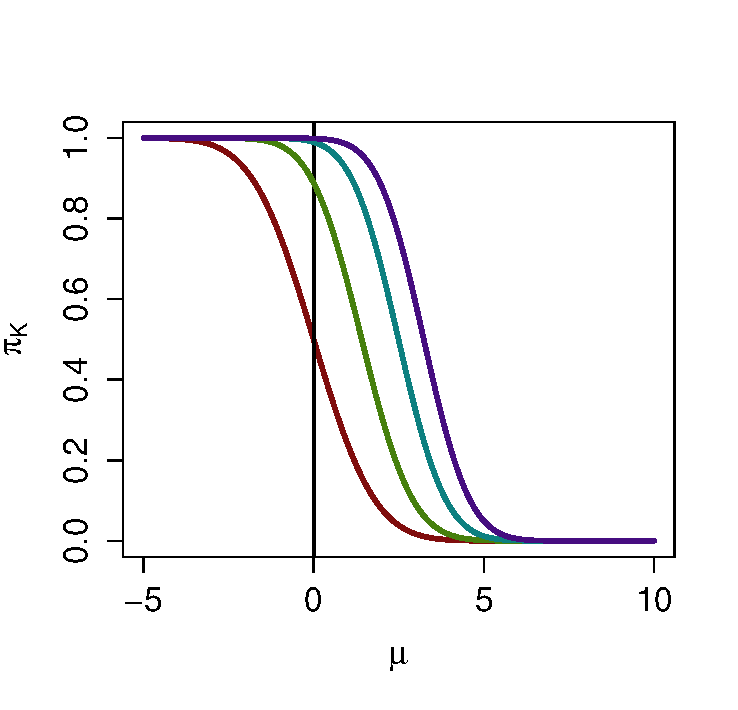
\includegraphics[scale = 0.5, clip=true, trim=0 0.2in 0 0.5in]{../info_theory_sims/illus_piK.pdf}
\caption{The function $pi_k(\mu)$, for $k = \{2, 9, 99, 999\}$ (left to right) \label{fig:pi}}
\end{figure}


First, let us rewrite $e_{ABE, k}$ in terms of the joint density $p(x, y)$.  Recall that the Bayes rule is
\[
e_{Bayes}(x_1,\hdots, x_k) = \frac{1}{k}\sum_{i=1}^k \Pr[\hat{X}(Y) \neq x_i| X = x_i].
\]
In turn, the Bayes classification rule is given in terms of the conditional density:
\[
\hat{X}(y) = \argmax_{x \in \{x_1,\hdots, x_k\}} p(y|x).
\]
Therefore, we obtain
\[
e_{Bayes}(x_1,\hdots, x_k) = \frac{1}{k}\sum_{i=1}^k \Pr[p(Y|x_i) \leq \max_{j \neq i} p(Y|x_j)| X = x_i].
\]
In turn the average Bayes error can be written as
\begin{align}
e_{ABE, k} &= \E[e_{Bayes}(X_1,\hdots, X_k)]
\\&= \frac{1}{k}\sum_{i=1}^k \E[\Pr[p(Y|x_i) \leq \max_{j \neq i} p(Y|x_j)| X = x_i]]
\\&= \E[\Pr[p(Y|x_1) \leq \max_{j \neq 1} p(Y|x_j)| X = x_1]]
\\&= \Pr[p(Y|X_1) \leq \max_{j \neq 1} p(Y|X_j)| X = X_1].
\end{align}

Defining $Z_i = \log p(Y|X_i) - \log p(Y|X_1)$, where $Y \sim p(y|X_1)$.
The we obtain
\[
e_{ABE} = \Pr[Z_1 < \max_{j > 1} Z_i].
\]

Our proof uses the assumption that $Z_1,\hdots, Z_k$ are asymptotically multivariate normal.
Supposing that $Z_1,\hdots, Z_k$ are indeed asymptotically normal, the following lemma
allows us to obtain a formula for the misclassification rate.

\textbf{Lemma 1. }
\emph{
Suppose $(Z_1, Z_2, \hdots, Z_k)$ are jointly multivariate normal, with 
$\E[Z_1 - Z_i]= \alpha$, 
$\Var(Z_1) = \beta$, 
$\Cov(Z_1, Z_i) = \gamma$, 
$\Var(Z_i)= \delta$, and $\Cov(Z_i, Z_j) = \epsilon$ for all $i, j = 2, \hdots,
k$, such that $\beta + \epsilon - 2\gamma > 0$.  Then, letting
\[
\mu = \frac{\E[Z_1 - Z_i]}{\sqrt{\frac{1}{2}\Var(Z_i - Z_j)}} = \frac{\alpha}{\sqrt{\delta - \epsilon}},
\]
\[
\nu^2 = \frac{\Cov(Z_1 -Z_i, Z_1 - Z_j)}{\frac{1}{2}\Var(Z_i - Z_j)} = \frac{\beta + \epsilon - 2\gamma}{\delta - \epsilon},
\]
we have
\begin{align*}
\Pr[Z_1 < \max_{i=2}^k Z_i] &= \Pr[W < M_{k-1}]
\\&= 1 - \int \frac{1}{\sqrt{2\pi\nu^2}} e^{-\frac{(w-\mu)^2}{2\nu^2}} \Phi(w)^{k-1} dw,
\end{align*}
where $W \sim N(\mu, \nu^2)$ and $M_{k-1}$ is the maximum of $k-1$
independent standard normal variates, which are independent of $W$.
}

[[proof in appendix]]

To see why the assumption that $Z_1,\hdots, Z_k$ are multivariate normal might be justified, suppose that $X$ and $Y$ have the same dimensionality $d$, and that
joint density factorizes as
\[
p(x_j, y) = \prod_{i=1}^d p_i(x_{j, i}, y_i)
\]
where $x_{j, i}, y_i$ are the components of $x_j$ and $y$.
Then,
\[
Z_i = \sum_{m=1}^d \log p_m(y_m | x_{m, i}) - \log p_m(y_m | x_{m, 1})
\]
where $x_{i, j}$ is the $i$th component of $x_j$.
The $d$ terms $\log p_m(y_m | x_{m, i}) - \log p_m(y_m | x_{m, 1})$ are independent across the indices $m$,
but dependent between the $i = 1,\hdots, k$.
Therefore, the multivariate central limit theorem can be applied to conclude that the vector
$(Z_1,\hdots, Z_k)$ can be scaled to converge to a multivariate normal distribution.
Now, since the average Bayes error $e_{ABE,k}$ is a continuous functional of the joint distribution $p(x, y)$,
it follows that $e_{ABE,k}$ converges to a functional of the limiting mean and covariance of $(Z_1,\hdots, Z_k)$, assuming
that the limits exist.
In our theorem, we assume a specific regime where these limits exist as a consequence.
While the componentwise independence condition is not a realistic assumption,
the key property of multivariate normality of $(Z_1,\hdots, Z_k)$ holds under more general conditions, and appears reasonable in practice.

The second component of our theorem is to manipulate the expression of the mutual information $I(X; Y)$.
The differential mutual information is defined as
\[
I(X; Y) = \int p(x, y) \log \frac{p(x, y)}{p(x) p(y)} dx dy.
\]
The key manipulation we employ is to approximate the logarithmic term by the Taylor expansion
\[
\log \frac{p(x, y)}{p(x) p(y)} \approx \frac{p(x, y) - p(x) p(y)}{p(x) p(y)} - \left(\frac{p(x, y) - p(x) p(y)}{p(x) p(y)}\right)^2 + \hdots.
\]
The approximation is accurate if $I(X; Y)$ is small--or rather, small relative to the dimensionality within the asymptotic sequence.
We state the theorem for the regime where $I(X; Y)$ is fixed, while the dimensionality of $X$ increases.

The asymptotic regime we consider is one where the dimension of $X$ goes to infinity.
This means that we have to consider a sequence of joint distributions $(X^{[d]}, Y^{[d]})$ indexed by the dimension $d$.

Fix integer $k \geq 2$.  Let $p^{[d]}(x,y)$ be a sequence of
probability density functions, where $x$ is of dimension $p^{[d]}$ and
$y$ is of dimension $q^{[d]}$.  Let $p^{[d]}(x)$ and $p^{[d]}(y)$
denote the marginal densities, and let
\[
p^{[d]}(y|x) = p^{[d]}(x, y)/p^{[d]}(y).\]
 Let $(X^{([d], i)}, Y^{([d], i)})$ be
iid random variates from $p^{[d]}(x, y)$ for $i = 1, \hdots, k$; we will supress the
superscripts $[d]$ and/or $(i)$ when convenient.  Recall the definitions of
entropy,
\[
H(X) = -\int p(x) \log p(x) dx,
\]
and mutual information
\[
I(X; Y) = \int p(x, y) \log \frac{p(x, y)}{p(x)p(y)} dx dy.
\]
Furthermore, define the $K$-class average Bayes error as
\[
e_{ABE, k} = \Pr[p(Y^{(1)}|X^{(1)}) < \max_{i = 2}^{k} p(Y^{(1)}|X^{(i)})].
\]
Define
\[
u^{[d]}(x, y) = \log p^{[d]}(x, y) - \log p^{[d]}(x) - \log p^{[d]}(y),
\]
and define
\[
\ell_{ij}^{[d]} = \log p(y^{(i)}|x^{(j)}).
\]



We now give the theorem and its proof.

\textbf{Theorem 1.} Let $p^{[d]}(x, y)$ be a sequence of joint densities
for $d = 1,2,\hdots$ as given above.  Further assume that
\begin{itemize}
\item[A1.] $\lim_{d \to \infty} I(X^{[d]}; Y^{[d]}) = \iota < \infty.$
\item[A2.] There exists a sequence of scaling constants $a_{ij}^{[d]}$
and $b_{ij}^{[d]}$ such that the random vector $(a_{ij}\ell_{ij}^{[d]} +
b_{ij}^{[d]})_{i, j = 1,\hdots, k}$ converges in distribution to a
multivariate normal distribution.
\item[A3.] There exists a sequence of scaling constants $a^{[d]}$, $b^{[d]}$ such that
\[
a^{[d]}u(X^{(1)}, Y^{(2)}) + b^{[d]}
\]
converges in distribution to a univariate normal distribution.
\item[A4.] For all $i \neq k$,
\[\lim_{d \to \infty}\Cov[u(X^{(i)}, Y^{(j)}), u(X^{(k)}, Y^{(j)})] = 0.\]
\end{itemize}
Then for $e_{ABE, k}$ as defined above, we have
\[
\lim_{d \to \infty} e_{ABE, k} = \pi_k(\sqrt{2 \iota})
\]
where
\[
\pi_k(c) = 1 - \int_{\mathbb{R}} \phi(z - c)  \Phi(z)^{k-1} dz
\]
where $\phi$ and $\Phi$ are the standard normal density function and
cumulative distribution function, respectively.

%[[Maybe add remark about assumptions here.]]

[Proof in supplemtn]

Assumptions A1-A4 are satisfied in a variety of natural models.
One example is a multivariate Gaussian sequence model where
\[
X \sim N(0, \Sigma_d)
\]
\[
E \sim N(0, \Sigma_e)
\]
\[
Y = X + E
\]
where $\Sigma_d$ and $\Sigma_e$ are $d \times d$ covariance matrices, and where $X$ and $E$ are independent.  Then, if $d \Sigma_d$ and $\Sigma_e$ have limiting spectra $H$ and $G$ respectively,
the joint densities $p(x, y)$ for $d = 1,\hdots, $ satisfy assumptions A1 - A4.

We can also construct a family of densities satisfying A1 - A4,
which we call an \emph{exponential family sequence model} since each joint distribution in the sequence
is a member of an exponential family: details are given in the supplement.
One example of such an exponential family sequence model is a multivariate logistic regression model,
given by
\[
X \sim N(0, I)
\]
\[
Y_i \sim \text{Bernoulli}(e^{\beta X_i}/(1 + e^{\beta X_i}))
\]
The multivariate logistic regression model (and multivariate Poisson regression model)
are especially suitable for modeling neural spike count data;
we simulate data from such a multivariate logistic regression model in section X.

Since $\pi_k$ is invertible for all $k = 2, \hdots$,
a converse relationship
\[
\lim_{d \to \infty} I(X^{[d]}; Y^{[d]}) = \frac{1}{2}(\pi_k^{-1}(\eta))^2
\]
also holds in the same regime.  We formally state the result, and a few consequences, as follows.

\textbf{Corollary 1.}
Let $p^{[d]}(x, y)$ be a sequence of joint densities
for $d = 1,2,\hdots$ as given above.  Further assume assumptions A2 - A4 and also
\begin{itemize}
\item[A1'.] $\lim_{d \to \infty} e_{ABE, k} = \eta < \infty.$
\end{itemize}
Then
\begin{itemize}
\item[i.]
\[
\lim_{d \to \infty} I(X^{[d]}; Y^{[d]}) = \frac{1}{2}(\pi_k^{-1}(e_{ABE}))^2.
\]
\item[ii.]
If $[\underline{e}, \bar{e}]$ is a $1-\alpha$ confidence interval for $e_{ABE, k}$,
then
\[
[\frac{1}{2}(\pi_k^{-1}(\bar{e}))^2, \frac{1}{2}(\pi_k^{-1}(\underline{e}))^2]
\]
is asymptotically a $1-\alpha$ confidence interval of $I(X; Y)$: that is,
\[
\lim_{d \to \infty} \Pr\left[I(X^{[d]}; Y^{[d]}) \in [\frac{1}{2}(\pi_k^{-1}(\underline{e}))^2, \frac{1}{2}(\pi_k^{-1}(\bar{e}))^2]\right] = 1-\alpha.
\]
\item[iii.] If $\hat{e}$ is a $O(1/\sqrt{n})$-consistent estimator for $e_{ABE, k}$,
and $\lim_{d \to \infty} e_{ABE, k} > 0,$
then $\frac{1}{2}(\pi_k^{-1}(\hat{e}))^2$ is a $O(1/\sqrt{n})$-consistent estimator for $I(X; Y)$.
\end{itemize}

[[Proof in appendix]]

As corollary 1 states, it is possible to construct a confidence interval for $I(X; Y)$ by
first constructing a confidence interval for the average Bayes error $e_{ABE,
k}$; then obtaining the confidence interval for $I(X; Y)$ as
\[
[\frac{1}{2}(\pi_k^{-1}(\bar{e}))^2, \frac{1}{2}(\pi_k^{-1}(\underline{e}))^2].
\]

Corollary 1 also gives the consisistent point estimate
\[\hat{I}(X; Y) = \frac{1}{2}(\pi_k^{-1}(\hat{e}))^2,\]
where $\hat{e}$ is a $O(1/\sqrt{n})$-consistent estimate of $e_{ABE,
k}.$ However, $\hat{I}(X, Y)$ may perform poorly in finite samples due
to bias.  Better performance can be obtained by using bias-correction
and shrinkage, but the optimality of the estimator depends on the
choice of risk function and risk criterion.  In the remainder
of the paper, we will be mainly interested in interval estimation.

\section{Results}

Multiple-response logistic regression model
\[
X \sim N(0, I_p)
\]
\[
Y \in \{0,1\}^q
\]
\[
Y_i|X = x \sim \text{Bernoulli}(x^T B_i)
\]
where $B$ is a $p \times q$ matrix.

\emph{Methods.}
\begin{itemize}
\item \text{Nonparametric}: $\hat{I}_0$ naive estimator, $\hat{I}_\alpha$ anthropic correction.
\item \text{ML-based}: $\hat{I}_{CM}$ confusion matrix, $\hat{I}_F$ Fano, $\hat{I}_{LS}$ low-SNR method.
\end{itemize}

Sampling distribution of $\hat{I}$ for \small{$\{p = 3$, $B = \frac{4}{\sqrt{3}} I_3$, $K = 20$, $r = 40\}$.}

True parameter $I(X; Y) = 0.800$ \emph{(dotted line.)}
\begin{center}
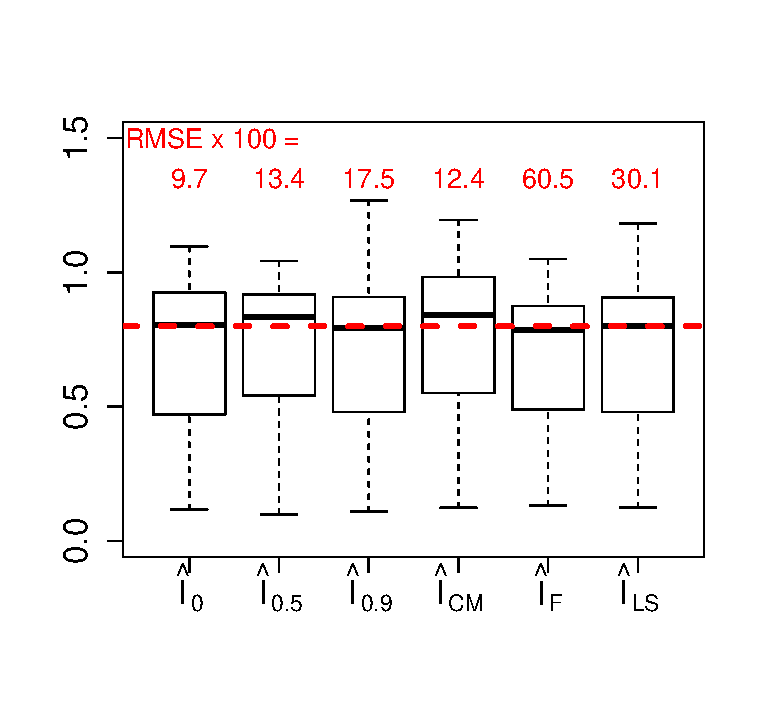
\includegraphics[scale = 0.5, clip = true, trim = 0 0.5in 0 0.5in]{../info_theory_sims/fig1.pdf}
\end{center}
Na\"{i}ve estimator performs best!  $\hat{I}_{LS}$ not effective.

Sampling distribution of $\hat{I}$ for \small{$\{p = 50$, $B = \frac{4}{\sqrt{50}} I_{50}$, $K = 20$, $r = 8000\}$.}

True parameter $I(X; Y) = 1.794$ \emph{(dashed line.)}
\begin{center}
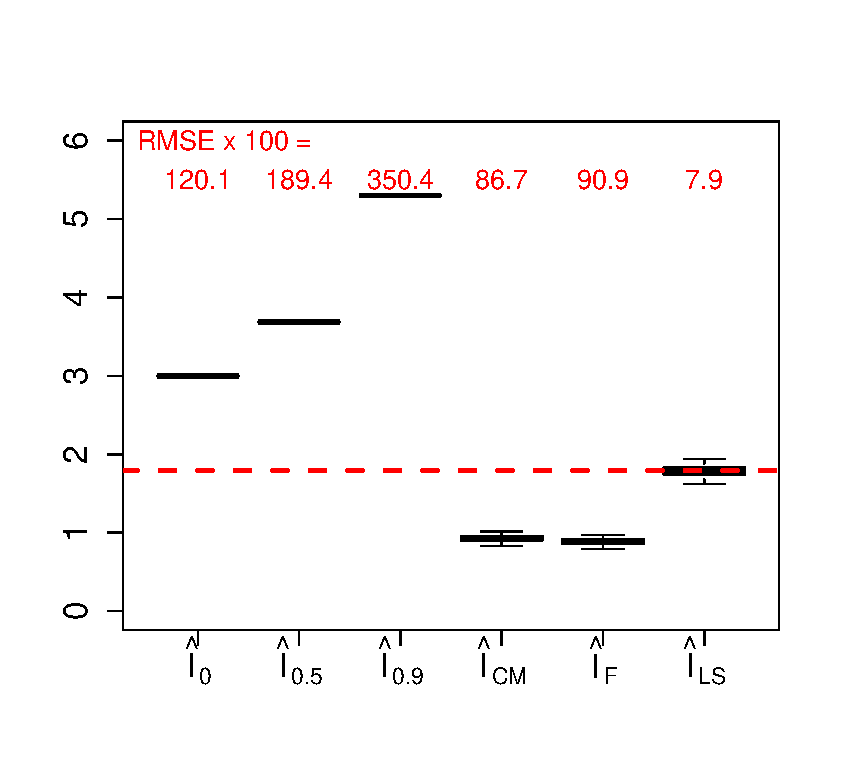
\includegraphics[scale = 0.5, clip = true, trim = 0 0.5in 0 0.5in]{../info_theory_sims/fig2.pdf}
\end{center}
Non-parametric methods extremely biased.

Estimation path of $\hat{I}_{LS}$ and $\hat{I}_\alpha$ as $n$ ranges from $10$ to $8000$.

\small{$\{p = 10$, $B = \frac{4}{\sqrt{10}} I_{10}$, $K = 20\}$.
True parameter $I(X; Y) = 1.322$ \emph{(dashed line.)}}

\begin{center}
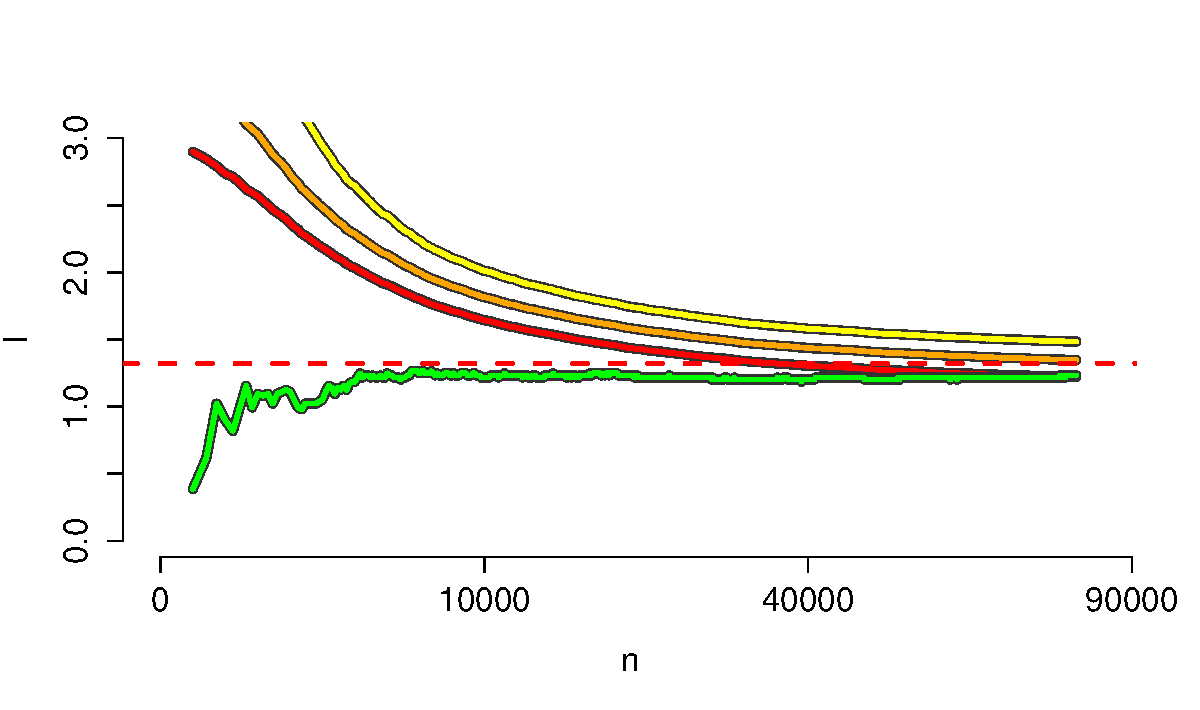
\includegraphics[scale = 0.4]{../info_theory_sims/fig3.pdf}
\end{center}

\begin{center}
\textbf{Estimated $\hat{I}$ vs true $I$.} 

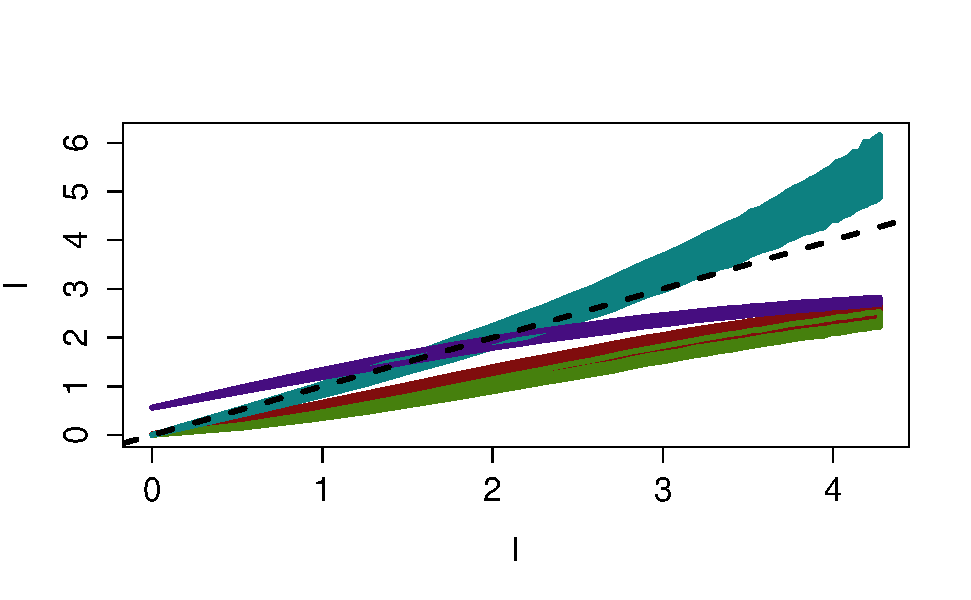
\includegraphics[scale = 0.5, clip=true, trim=0.4in 0.5in 0 0.5in]{../info_theory_sims/fig4.pdf}
\end{center}

Sampling distribution of $\hat{I}_{LS}$ for \small{$\{p = 10$, $B = \frac{4}{\sqrt{10}} I_{10}$, $N = 80000\}$,

and $K = \{5, 10, 15, 20, \hdots, 80\}$, $r = N/k$.}

True parameter $I(X; Y) = 1.322$ \emph{(dashed line.)}
\begin{center}
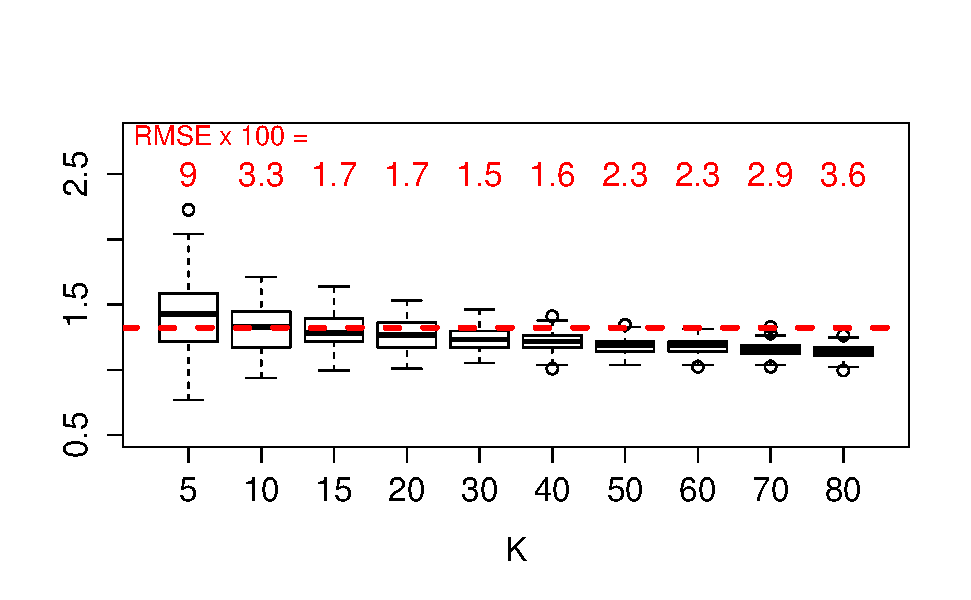
\includegraphics[scale = 0.6, clip = true, trim = 0 0.5in 0 0.5in]{../info_theory_sims/fig5a.pdf}
\end{center}

Decreasing variance as $K$ increases. Bias at large and small $K$.

$p = 20$ and $q = 40$, entries of $B$ are iid $N(0, 0.025)$.

$K=20$, $r = 8000$, true $I(X; Y) = 1.86$ \emph{(dashed line.)}

\begin{center}
\textbf{Sampling distribution of $\hat{I}$.}
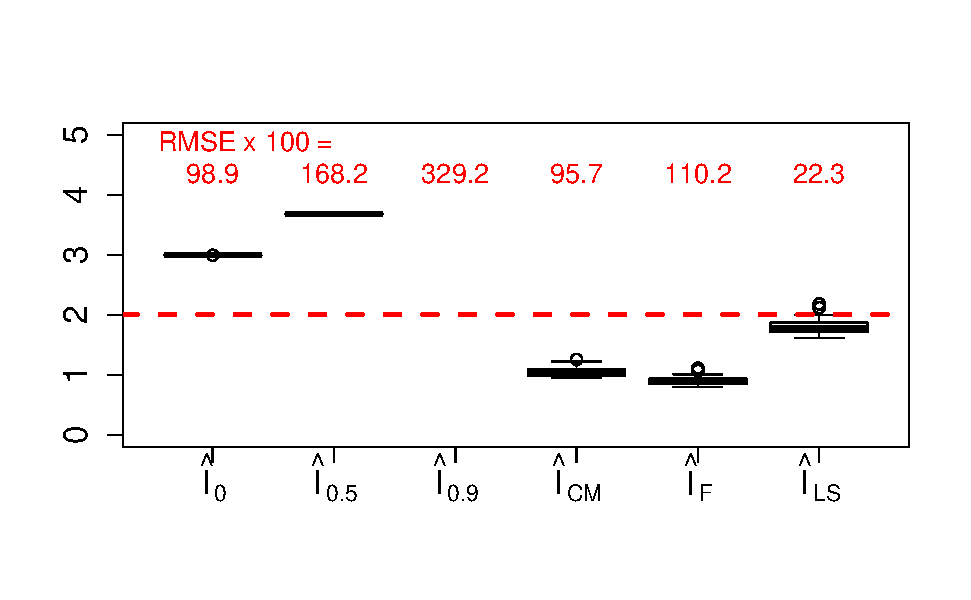
\includegraphics[scale = 0.6, clip = true, trim = 0 0.5in 0 0.5in]{../info_theory_sims/fig6.pdf}
\end{center}

\section{Discussion}

\subsubsection*{Acknowledgments}

Use unnumbered third level headings for the acknowledgments. All
acknowledgments go at the end of the paper. Do not include
acknowledgments in the anonymized submission, only in the final paper.

\section*{References}

References follow the acknowledgments. Use unnumbered first-level
heading for the references. Any choice of citation style is acceptable
as long as you are consistent. It is permissible to reduce the font
size to \verb+small+ (9 point) when listing the references. {\bf
  Remember that you can use a ninth page as long as it contains
  \emph{only} cited references.}
\medskip

\small

[X] Gastpar, M.  Gill, P.  Huth, A.  Theunissen, F. ``Anthropic Correction of Information Estimates and Its Application to Neural Coding.'' \emph{IEEE Trans. Info. Theory}, Vol 56 No 2, 2010.

[X] A. Borst and F. E. Theunissen, ``Information theory and neural coding''
Nature Neurosci., vol. 2, pp. 947?957, Nov. 1999.

[X] L. Paninski, ``Estimation of entropy and mutual information,'' Neural
Comput., vol. 15, no. 6, pp. 1191?1253, 2003.

[X] I. Nelken, G. Chechik, T. D. Mrsic-Flogel, A. J. King, and J. W. H.
Schnupp, ``Encoding stimulus information by spike numbers and mean
response time in primary auditory cortex,'' J. Comput. Neurosci., vol.
19, pp. 199?221, 2005.

[X] Cover and Thomas.  Elements of information theory.

[X]  Muirhead.  Aspects of multivariate statistical theory.

[X] van der Vaart.  Asymptotic statistics.

[1] Alexander, J.A.\ \& Mozer, M.C.\ (1995) Template-based algorithms
for connectionist rule extraction. In G.\ Tesauro, D.S.\ Touretzky and
T.K.\ Leen (eds.), {\it Advances in Neural Information Processing
  Systems 7}, pp.\ 609--616. Cambridge, MA: MIT Press.

[2] Bower, J.M.\ \& Beeman, D.\ (1995) {\it The Book of GENESIS:
  Exploring Realistic Neural Models with the GEneral NEural SImulation
  System.}  New York: TELOS/Springer--Verlag.

[3] Hasselmo, M.E., Schnell, E.\ \& Barkai, E.\ (1995) Dynamics of
learning and recall at excitatory recurrent synapses and cholinergic
modulation in rat hippocampal region CA3. {\it Journal of
  Neuroscience} {\bf 15}(7):5249-5262.

\end{document}
